\documentclass[a4paper,12pt,fleqn]{scrartcl}%fleqn pour aligner les equations à gauche
\usepackage{../../Styles/Cours}

\newcommand{\chnum}{Chapitre 13}
\newcommand{\chtitle}{Mouvement des astres et des planètes}
\newcommand{\dtype}{Cours}

\begin{document}
\maketitle

\section{Étude d'un mouvement orbital simple}
	\subsection{Accélération et repère de Frenet (rappels)}
	\begin{minipage}{.72\linewidth}
	En cinématique, le repère de Frenet est un outil d'étude permettant d'exprimer plus facilement les vecteurs vitesse et accélération d'un système $M$ en mouvement.\\
	A retenir :
	\begin{itemize}
		\item Les vecteurs $\vec{T}$ (tangentiel) et $\vec{N}$ (normal) sont unitaires (norme = 1) et orthogonaux entre eux.
		\item Le vecteur vitesse d'un mobile est toujours tangent à la trajectoire : \fbox{$\vec{v} = v \cdot \vec{T}$}
		\item Le vecteur accélération s'écrit dans le repère de Frenet : \fbox{$a_N \cdot \vec{N} + a_T \cdot \vec{T}$}
		\item $\text{avec : } \begin{array}{l} 
		a_N \text{ l'accélération normale telle que : } a_N = \dfrac{v^2}{R}\\
		a_T \text{ l'accélération tangentielle telle que : } a_T =\dfrac{dv}{dt}
		\end{array}$
	\end{itemize}
\end{minipage}
\begin{figure}[h!]
	\begin{minipage}{.7\linewidth}
	\begin{tcolorbox}[arc=1ex, colframe=black, left=3pt, right=3pt, top=3pt, bottom=2pt]
	\textbf{Exemple 1 :}\\
	Définir les conditions nécessaires sur $a_N$ et $a_T$ pour :
		\begin{itemize**}
			\item Un mouvement rectiligne et uniforme
			\item Un mouvement circulaire et uniforme
			\item Un mouvement rectiligne accéléré
		\end{itemize**}
	\end{tcolorbox}	
	\end{minipage}
\end{figure}

	\subsection{Nature du mouvement}
	\begin{minipage}{.7\linewidth}
	Le mouvement d'un objet en orbite autour d'un astre est toujours une ellipse. Dans certains cas, cette ellipse est un cercle ou s'en rapproche fortement, comme par exemple pour l'orbite de la Terre dans le référentiel héliocentrique.\\
	Considérons le mouvement circulaire de la Terre autour du Soleil :\\ 
	\begin{tabular}{m{.4\linewidth} m{.5\linewidth}}
	\textbf{Système étudié} & Terre de masse $M_T$\\
	\textbf{Référentiel d'étude :} & Héliocentrique supposé galiléen\\
	\textbf{Inventaire des forces :} & Force d'interaction gravitationnelle exercée par le Soleil sur la Terre\\	
	\end{tabular}\\
	Comme la masse de la Terre est constante, d'après la deuxième loi de Newton, on a :
	\begin{eqnarray}
	\sum \vec{F} = \vv{F_{S/T}} = M_T \cdot \vec{a} \nonumber
	\end{eqnarray}
	Or, la force exercée par le Soleil de masse $M_S$ sur la Terre a pour expression :\\
	\begin{tabular}{m{4cm}|m{4cm}}
	\multirow{4}{4cm}{$\vv{F_{S/T}} = G \cdot \dfrac{M_T M_S}{R^2}\cdot \vec{N}$}
	&$F \text{ en } \unit{\newton}$\\
	&$M \text{ en } \unit{\kilo \gram}$\\
	&$R \text{ en } \unit{\meter}$\\
	&$G = \num{6,6710e-11} \text{ SI}$\\
	\end{tabular}\\
	D'où : 
	$$\vec{F} = M_T \cdot \vec{a} $$
	$$\leftrightarrow  \cdot \dfrac{M_T M_S}{R^2}\cdot \vec{N}  = M_T \left(a_N \cdot \vec{N} + a_T \cdot \vec{T} \right)$$
	$$\leftrightarrow  G \cdot \dfrac{M_T M_S}{R^2}\cdot \vec{N}  = M_T \cdot a_N \cdot \vec{N} + M_T \cdot a_T \cdot \vec{T}$$
	Par identification :$$M_T \cdot a_N = G \cdot \dfrac{M_T M_S}{R^2}$$
	$$\leftrightarrow a_N = G \cdot \dfrac{M_S}{R^2}$$
	$$ a_T = 0$$
	Or, si $a_T=0$ alors $\dfrac{dv}{dt}=0$ car par définition $a_T=\dfrac{dv}{dt}$\\
	Donc $v=cste$.\\
	Ainsi, si la trajectoire d'un objet en orbite gravitationnelle est circulaire, alors son mouvement est nécessairement uniforme.\\
	Exemple : la Terre ayant une orbite quasi-circulaire, sa vitesse reste toujours voisine de \num{30} \unit{\kilo \meter \per \second}.
	\end{minipage}
	
	\subsection{Vitesse orbitale}
	D'après la partir précédente, on a : $a_N = G \cdot \dfrac{M_S}{R^2}$\\
	Par définition $a_N = \dfrac{v^2}{R}$\\
	On peut donc écrire que :\\
	\begin{tabular}{m{8cm}|m{8cm}}
	\multirow{4}{8cm}{$\dfrac{v^2}{R}=G \cdot \dfrac{M_S}{R^2} \leftrightarrow v = \sqrt{G \cdot \dfrac{M_S}{R}}$}&$R \text{ en } \unit{\meter}$\\
	&$ v \text{ en } \unit{\meter \per \second}$\\
	&$M_S \text{ en } \unit{\kilo \gram}$\\
	&$G = \num{6,6710e-11} \text{ SI}$\\
	\end{tabular}
	\subsection{Période de révolution}
	La période de révolution $T$ d'un astre est le temps nécessaire à ce dernier pour effectuer un tour autour de l'astre qui le maintient en orbite. Par exemple, la période de révolution de la Terre autour du Soleil est de un an.\\ En considérant que l'orbite de la Terre est un cercle, la longueur $L$ de cette orbite est donc le périmètre du cercle de rayon $R$ :
	$$	L = 2 \pi \cdot R $$
	La vitesse $v$ de la Terre sur son orbite étant constante, sa valeur instantanée est à chaque instant égale à sa valeur moyenne, donc :
	$$v = \dfrac{d}{\Delta t} = \dfrac{L}{T} = \dfrac{2 \pi \cdot R}{T}$$
	$$\leftrightarrow \sqrt{G \cdot \dfrac{M_S}{R}} = \dfrac{2 \pi R}{T}$$
	$$\leftrightarrow T = 2 \pi \sqrt{\dfrac{R^3}{GM_S}}$$
	À noter : l'orbite géostationnaire (GEO pou GEostationary Orbit) est une orbite circulaire dans le plan équatorial de la Terre de période orbitale égale à la période de rotation de la Terre, soit \num{23} \unit{\hour} \num{56} \unit{\minute} \num{4} \unit{\second}. Un objet placé sur une telle orbite reste en permanence au-dessus du même point de l’Équateur.
\section{Lois de Kepler}
	\subsection{Loi des orbites (première loi de Kepler - 1609)}
	\begin{minipage}{.7\linewidth}
	Dans le référentiel héliocentrique, la trajectoire des planètes est une ellipse dont l'un des foyers est le centre du Soleil.\\
	On note : 
	\begin{itemize*}
		\item le péricentre est le point de l'orbite le plus proche de l'astre central. Si l'astre est le Soleil, on parle de périhélie. Pour la Terre, c'est le périgée.
		\item l'apocentre est le point de l'orbite le plus éloigné de l'astre central. Si l'astre central est le Soleil, on parle plus précisément d'aphélie. Pour la Terre, c'est l'apogée.
		\item $a$ est le demi-grand-axe et $b$ est le demi-petit axe
	\end{itemize*}
	\end{minipage}
	\begin{minipage}{.3\linewidth}
	\begin{center}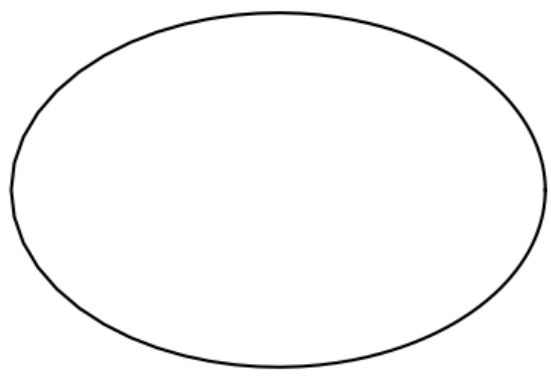
\includegraphics[width=\linewidth]{Ressources/TSPE_C6_Fig2.png} \end{center}
	\end{minipage}
	\subsection{Loi des aires (deuxième loi de Kepler - 1609)}
	\begin{minipage}{.7\linewidth}
	Le segment $[SP]$ qui relie le centre du Soleil au centre de la planète balaie des aires égales pendant des durées égales.\\
	Cette loi implique que plus la planète s'approche du Soleil plus sa vitesse augmente. De même, plus elle s'en éloigne, plus sa vitesse diminue.
	\end{minipage}
	\begin{minipage}{.3\linewidth}
	\begin{center}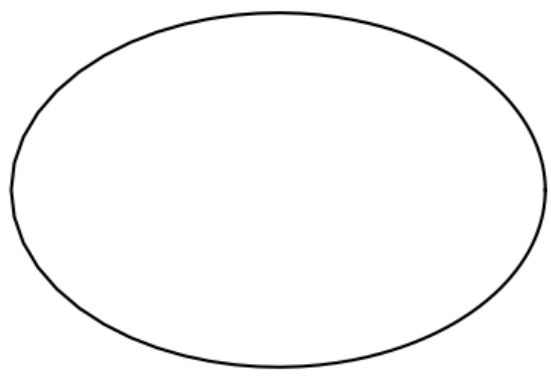
\includegraphics[width=\linewidth]{Ressources/TSPE_C6_Fig2.png} \end{center}
	\end{minipage}
	\subsection{Loi des périodes (troisième loi de Kepler - 1618)}
	Le carré de la période de révolution d'une planète est proportionnel au cube du demi grand axe de son orbite.
	$$T^2 = k \times a^3 \leftrightarrow \dfrac{T^2}{a^3} = k $$
	avec $k$ une constante.

 
	\begin{figure}[h!]
	\begin{tcolorbox}[arc=1ex, colframe=black, left=3pt, right=3pt, top=3pt, bottom=2pt]
	\textbf{Exemple 2 :}\\
	En partant de la formule ci-après, rechercher l'expression de la constante $k$ en fonction de $G$ et $M_S$.
	$$	T=2 \pi \sqrt{\dfrac{R^3}{GM_S}} $$
	\end{tcolorbox}	
	\end{figure}

 
\end{document}